\chapter{Introduction: Why the Relevant Energy Range Changes with Mission Domain}

\subsection{Characterising the Space Enviroment}

\begin{figure}[htbp]
	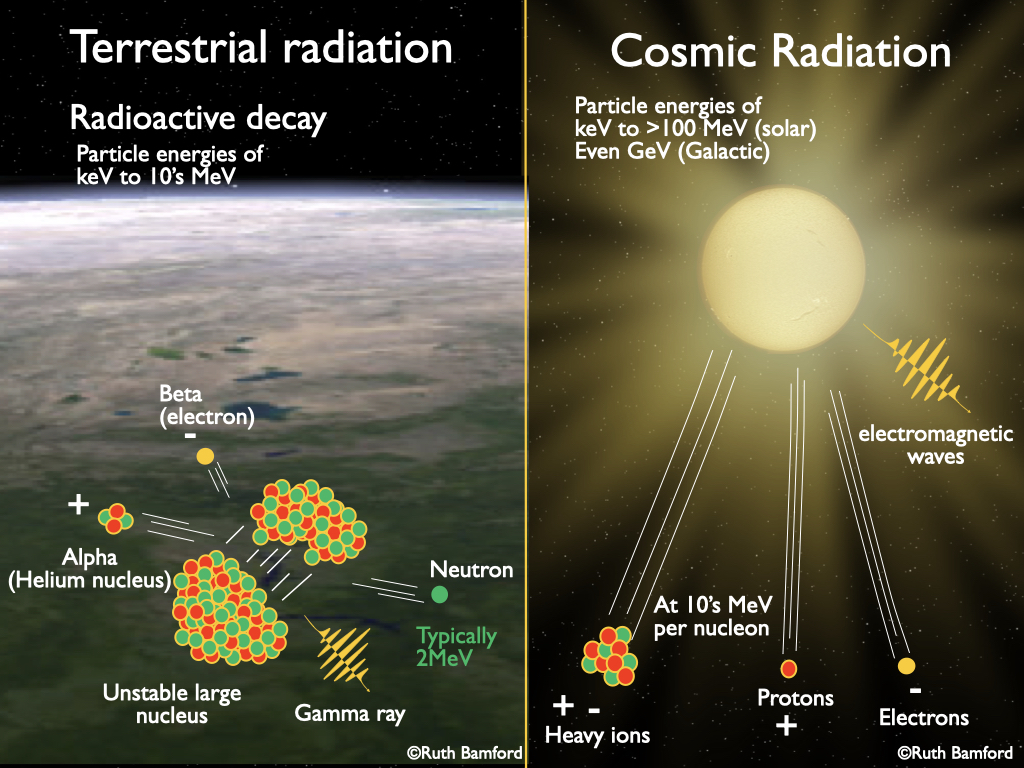
\includegraphics[width=0.45\textwidth]{FIGURES/DifferentTypesRadiation.jpeg}
	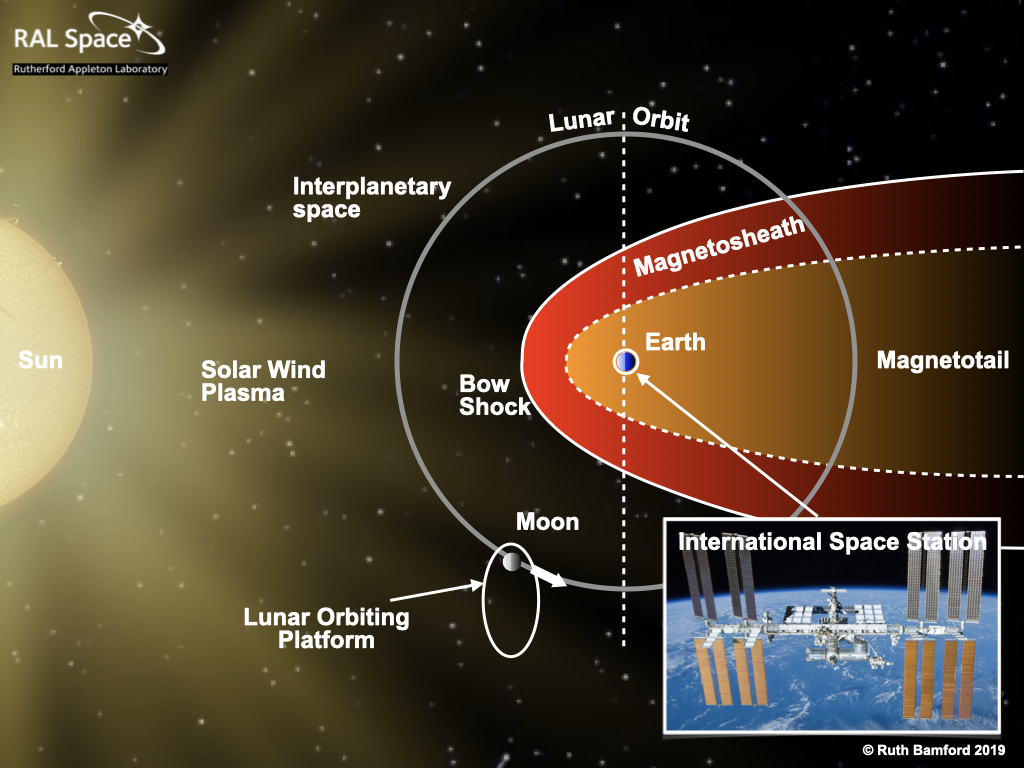
\includegraphics[width=0.45\textwidth]{FIGURES/LunarOrbit.jpeg}
	\caption{(left) The radiation in space is very different from type of radiation encountered from terrestrial source other than cosmic rays.
	(Right) The Moon orbits in and out of the Earth's magnetosphere and therefore has a complex and varied plasma environment. 
	}
	\label{fig:DifferentTypesRadiation}
\end{figure}

The number and velocity of ions and electrons in space is changing all the time.
The ions and electrons of space are quasi-neutral (a plasma) and originate from the Sun predominantly (Solar `cosmic rays' SCR) but also violent events such as supernova and others from  galactic sources and beyond(Galactic `cosmic rays' GCR).

During periods of enhanced solar activity, such as solar flares and coronal mass ejections (CMEs), the flux of energetic charged particles can increase dramatically by many orders of magnitude, through Solar Energetic Particle (SEP) events. At even higher energies, Galactic Cosmic Rays (GCRs), believed to originate primarily from supernova remnants and other energetic astrophysical sources within our Galaxy, provide a persistent background radiation environment. 

SEPs form a primarily concern to spacecraft operators (and astronauts) as they arrive suddenly without warning and contain highly penetrating ions and electrons. With CMEs there is some warning as it takes time for the plasma `cloud' to reach Earth and it can be detected by monitoring spacecraft.

The Earth's magnetosphere changes the energy distribution of some of the ions and electrons but not all. Some are so energetic they pass straight through the magnetic boundaries. Others The become trapped within the Van Allen radiation belts.

The radiation of space is different in character to that encountered terrestrially other than cosmic rays. This is illustrated in Figure~\ref{fig:DifferentTypesRadiation}(far left and middle). 

\begin{figure}[htbp]
	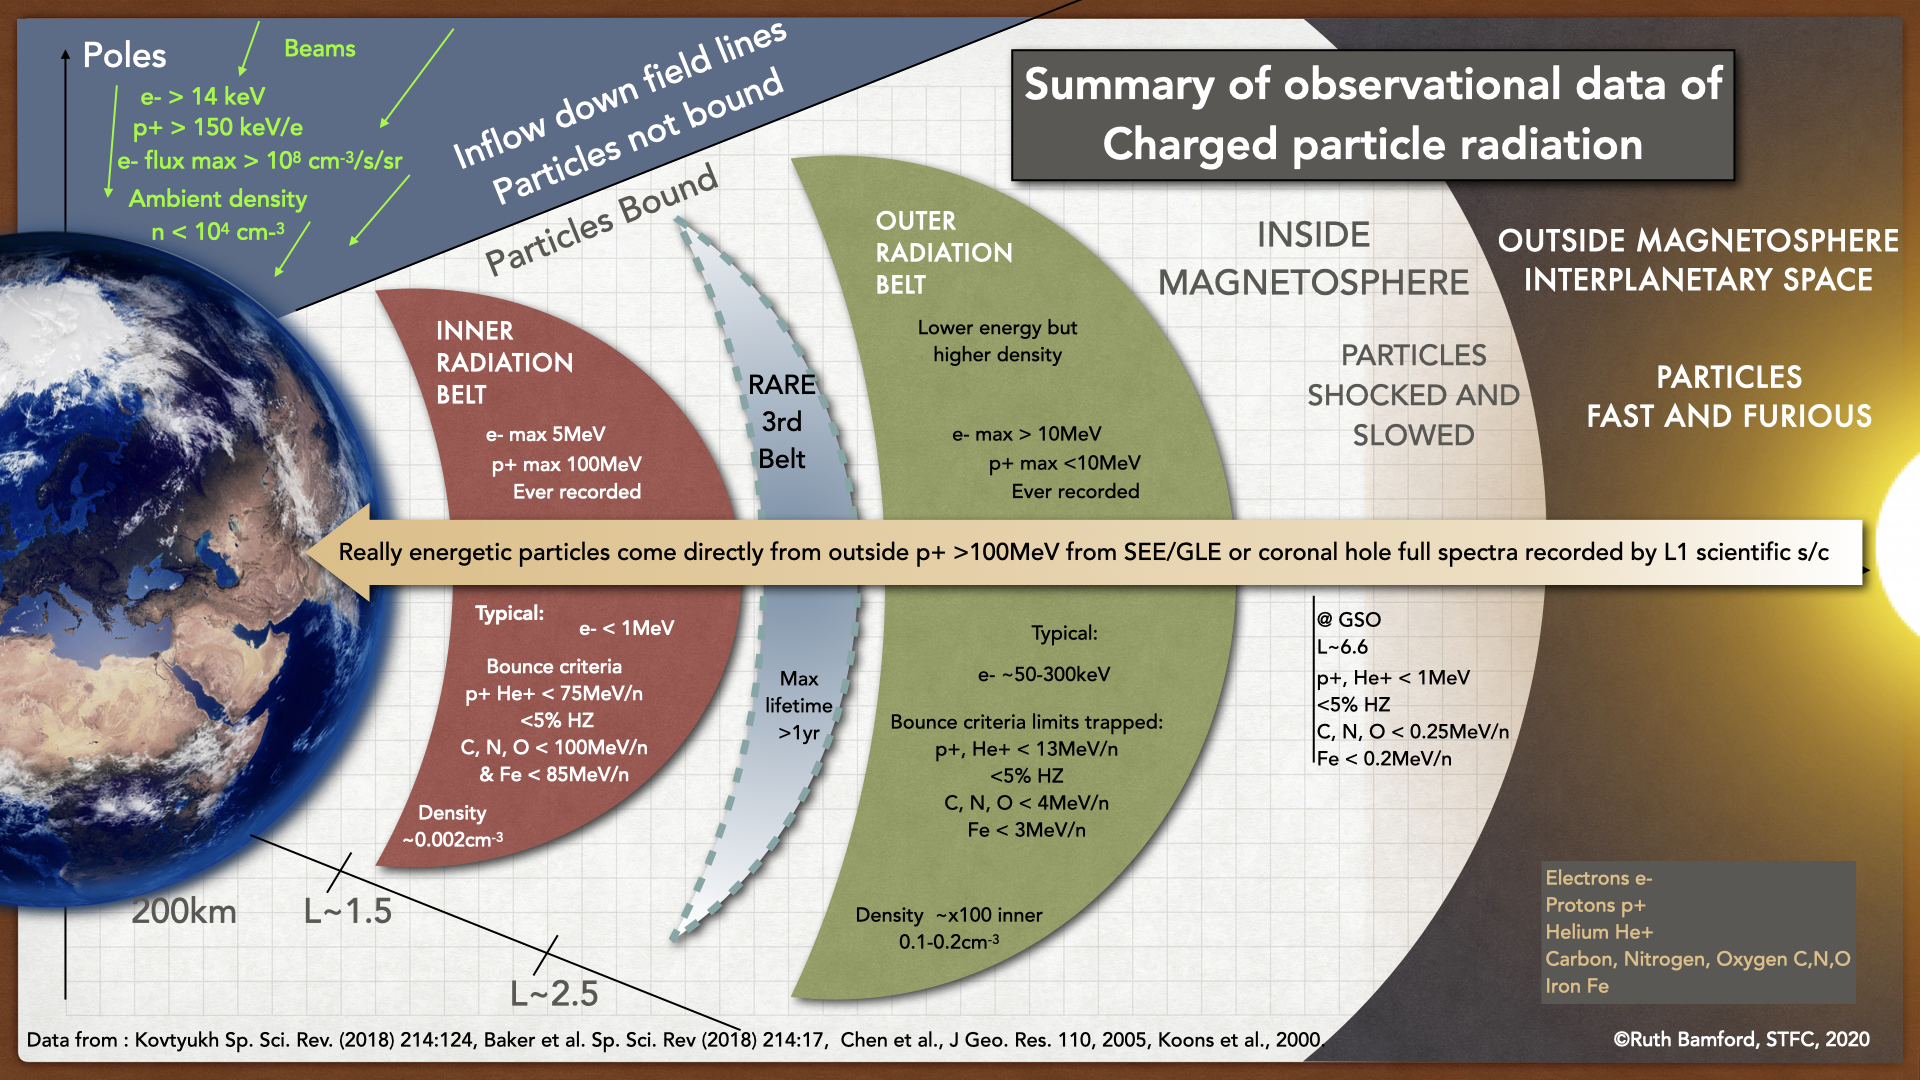
\includegraphics[width=1.0\textwidth]{FIGURES/Rad_Data_Summary_ImageSWIMMR.jpeg}
	\caption{A graphically summary of the trapped and passing energy range of plasma particles expected within each region of the near Earth environment. Source data includes Kovtyukh Sp.Sci. Rev. (2018) 214:124, Baker et al. Sp. Sci. Rev (2018) 214:7, Chen et al., J. Geo. Res. 110, (2005) and Koons et. al., (2000). \cite{Kovtyukh2018, Baker2018, Koons2000}. 
	}
	\label{fig:Enviroments}
\end{figure}

\paragraph{The Moon as emerging market}
The Moon orbits in and out of the Earth's magnetosphere and therefore has a complex and varied plasma environment as is shown in the far right hand panel Figure~\ref{fig:DifferentTypesRadiation}. For the majority of the orbit however spacecraft on or in orbit are outside the Earth's magnetosphere. Low cost sophisticated, multiple gravity assist orbits are what are opening the Moon as destination to commercial flyers.

The lunar environment is considerably more complex than either low Earth orbit or deep interplanetary space. During its 27.3-day orbit, the Moon periodically passes through the Earth's magnetotail before returning to the ambient solar wind. This is illustrated in the furthest right image in Figure~\ref{fig:DifferentTypesRadiation}. As a consequence, spacecraft operating in cislunar space or lunar orbit experience a changing radiation environment, alternating between geomagnetic influence and direct exposure to the interplanetary particle population. For the majority of each orbit, however, the Moon lies outside the Earth's protective magnetosphere and is exposed directly to solar energetic particles, galactic cosmic rays and locally generated secondary particles.



Table~\ref{tab:domains} summarises the principal radiation environments encountered by spacecraft together with the corresponding engineering measurement requirements. The near Earth environments are illustrated graphically in Figure~\ref{fig:Enviroments}.



\begin{table}[htbp]
\centering
\caption{Summary of radiation-monitor requirements by mission domain. Values are indicative rather than universal boundaries.}
\label{tab:domains}
\small
\ReportTableRows
\begin{tabularx}{\textwidth}{p{1.45cm} p{3.1cm} p{3.1cm} X}
\toprule
\rowcolor{RALblue}
\tablehead{Domain} & \tablehead{Principal populations} & \tablehead{Energy concerns} & \tablehead{Engineering consequence} \\
\midrule
LEO & Trapped protons, electrons, South Atlantic Anomaly, atmospheric secondaries & Electrons from keV to MeV; protons from MeV to hundreds of MeV & Large changes with altitude and inclination; high count rates in belt crossings; dose, displacement damage, charging and single-event effects. \\
MEO & Inner and outer radiation belts; persistent energetic electrons; trapped protons & Electrons from hundreds of keV to several MeV; protons from MeV to hundreds of MeV & Long-duration GNSS exposure requires stable calibration, wide dynamic range and charging measurements. \\
GEO & Outer-belt electrons, solar energetic particles, cosmic-ray background & Electrons from tens of keV to several MeV; SEP protons from MeV to hundreds of MeV and above & Operational monitoring requires continuous telemetry, directional response information and contamination control. \\
HEO & Repeated belt traversals plus solar-particle exposure & Broad electron and proton coverage, rapidly changing flux & High dynamic range and discrimination across very different environments within one orbit. \\
Interplanetary & Solar wind, SEP, GCR and heavy ions & keV solar-wind plasma through GeV/nucleon GCR & Particle identification and high-energy response become increasingly important. \\
Cislunar & SEP, GCR, solar wind, magnetotail intervals, albedo particles and secondary neutrons/gamma rays & keV to GeV; charged and neutral secondaries & Compact multi-species monitors, directional measurements and neutron capability become more valuable. \\
\bottomrule
\end{tabularx}
\StopReportTableRows
\end{table}
%%%%%%%%%%%%%%%% End of Environments %%%%%%%%%



\begin{table}[htbp]
\centering
\caption{Why different particle and energy channels are required.}
\small
\ReportTableRows
\begin{tabularx}{\textwidth}{p{2.0cm} p{2.9cm} p{3.6cm} X}
\toprule
\rowcolor{RALblue}
\tablehead{Quantity} & \tablehead{Indicative range} & \tablehead{Primary engineering relevance} & \tablehead{Typical measurement approach} \\
\midrule
Low-energy electrons & eV--100 keV & Surface charging; plasma environment & Electrostatic analyser or filtered solid-state detector \\
Energetic electrons & 0.1--20 MeV & Internal charging, total dose, space-weather operations & Silicon telescope, scintillator or pixel detector \\
Protons & 0.1--500 MeV and above & Dose, displacement damage, SEE, SEP monitoring & Silicon stack, scintillator telescope or hybrid calorimeter \\
Alpha particles & MeV/n to hundreds of MeV/n & SEP composition, dose and particle identification & Multi-layer $\Delta E$--$E$ telescope \\
Heavy ions & $\sim$10 MeV/n to GeV/n & High-LET events and single-event effects & Silicon stack, magnetic spectrometer or calorimeter \\
Neutrons & Thermal to hundreds of MeV & Secondary radiation and dose equivalent & Converter plus scintillator or semiconductor \\
Gamma rays & keV--MeV and above & Secondary environment and spectroscopy & Scintillator or semiconductor spectrometer \\
Dose / LET & Mission-dependent & Crew exposure, electronics qualification, shielding validation & TEPC, silicon dosimeter, passive dosimeter or LET telescope \\
Charging current & fA--pA cm$^{-2}$ scale & Internal dielectric charging and anomaly diagnosis & Shielded charge plates or dedicated charging monitor \\
\bottomrule
\end{tabularx}
\StopReportTableRows
\end{table}
